\chapter{Process en resultaten}
In dit hoofdstuk beschrijf ik het proces en de resultaten van het afstudeerproject. Bij afwijkingen van het originele plan dat beschreven in het Plan Van Aanpak is dit beargumenteerd. Verder wordt er in dit hoofdstuk alleen het proces en de resultaten geconstateerd. Reflectie hierop en mijn keuzes worden in een volgend hoofdstuk beschreven en in dit hoofdstuk constateer ik alleen wat er is gebeurd.

\section{Verloop van het project}
Om het verloop van het project gestructureerd te verwoorden, is het project te verdelen in 4 fases: Initiatie fase, definitie fase, analyse en realisatie fase en afronding fase. Dit zijn ook de fases die opgenomen zijn in de planning in het plan van aanpak en zijn in de onderstaande subparagrafen op chronologische volgorde beschreven.\par

Door de agile aanpak is in derde fase er beide analyse en realisatie tegelijkertijd uitgevoerd.  De gekozen Kanban agile methode laat dit ook toe. De reden hiervoor is om risico’s van het project te verminderen door de software, het onderzoek en enige analyse tegelijkertijd stukje voor stukje uit te voeren in iteraties \footnote{https://www.twynstraguddekennisbank.nl/projectmanagement/faseer-het-project}.

\subsection{Fase: Initiatieffase (iteratie 0)}
In deze eerste fase is het doel om een gelijk beeld van het project te verkrijgen van alle betrokkenen aan het project en hiermee goedkeuring te krijgen om het project te starten. Dit is gedaan door de stand van zaken vast te stellen en onderzoek te doen naar de aanleiding en doelstelling van het project.\par

Deze fase is samen met de definitiefase uitgevoerd waar verdere analyse is gedaan naar het te ontwikkelen product. Dit is gedocumenteerd in het Plan Van Aanpak waarin het beoogde projectresultaat in termen van: randvoorwaarden, functionele en operationele prestaties, eisen, wensen en projectgrenzen duidelijk wordt. Een planning in de vorm van een GANTT chart met daarin de deadlines die vanuit school bekend zijn, geeft een beeld voor de komende fases.
\newpage

\subsection{Fase 2: Definitiefase (iteratie 0 - 1)}
In de tweede fase is er verder gekeken naar het te ontwikkelen product. In deze fase is het Plan van Aanpak verder afgerond en vervolgens goedgekeurd, door zowel de stagebegeleider en assessor als de bedrijfsbegeleider. De ontwikkelmethode, Kanban is gekozen en de planning voor de aankomende realisatie- en analysefase zijn opgesplitst in 7 iteraties van 2 weken. Daarbij wordt per iteratie gekeken naar wat er nodig is aan werk voor de komende 2 weken.\par

Om te beginnen is het duidelijk dat er een onderzoek gestart moet worden. De aanleiding hiervoor is dat het doel van het proof of concept moet aantonen dat het elektronische claim systeem use case van Allianz met de Blockchain Technologie geautomatiseerd kan worden.\par

Omdat ik zelf nog niet bekend ben met de Blockchain Technologie en het duidelijk is dat er in een later stadium een geïnformeerd besluit gemaakt over moet worden, is het duidelijk dat de eerste iteratie zich vooral bezighoudt met een algemeen onderzoek naar de Blockchain Technologie. Hiermee is de definitiefase afgerond en begint de analyse / realisatie fase. 

\subsection{Fase 3: Analyse / Realisatie Fase (Iteraties 1 - 5)}
Er is tijdens deze fase meerdere malen analyse en realisatie uitgevoerd. In de onderstaande subparagrafen beschrijf ik per iteratie hoe het proces is gelopen en waar aan gewerkt is. De grootste afwijking met het originele plan, in het plan van aanpak is het opsplitsen van de resultaten in het onderzoeksverslag dat bestaat uit een literatuuronderzoek, analyse en het proof of concept experiment. Dit wordt gedaan na het ontvangen van de feedback op de 80\% versie en om verwarring te vermijden wordt er in het proces hieronder verwezen naar de namen van de losse documenten die aan het einde van het project met dit afstudeerverslag zijn meegeleverd.
\newpage

\subsubsection{Iteratie 1 - Onderzoek naar Blockchain en huidige proces}
In de eerste iteratie is er gekeken naar hoe het huidige claim proces werkt. Deze analyse vult de analyse die is gestart voor het Plan van Aanpak aan met gesprekken met de opdrachtgever Allianz Group en de Product Owner. Uit deze analyse zijn requirements opgesteld en user stories en actoren van het te ontwikkelen proof of concept gedocumenteerd in het Software Architecture Document. (SD-1, SD-2)\par

Daarnaast is er een literatuuronderzoek uitgevoerd naar een technische basis termen rondom de blockchain-technologie en gerelateerde onderwerpen. Dit is gedaan om een aantal basis technische termen in cryptografie, blockchain-technologie en gerelateerde onderwerpen duidelijk te krijgen. Hiermee weet ik waar ik het over heb wanneer het proof of concept in vervolg iteraties behandeld wordt.\par

De focus is met name de manier waarop de blockchain gebruikt zou kunnen worden voor het doeleinde van de klant. Tijdens de eerste week is al snel duidelijk dat er verschillende types Blockchains zijn: Consortium, Privé en openbaar, en die zijn vervolgens onderzocht. (SD-7)
\newpage
\subsubsection{Iteratie 2 - Onderzoek naar de architectuur van de blockchain en smart contracts}
Tijdens de tweede iteratie is er verder onderzoek uitgevoerd naar de blockchain technologie en is het uitgebreid naar Smart Contracts en de blockchain zijn architectuur. Dit allemaal om duidelijk te krijgen hoe hiermee een gedecentraliseerde blockchain applicatie (Dapps \footnote{https://en.wikipedia.org/wiki/Decentralized\_application}) ontwikkeld zou kunnen worden.\par

Verder is het onderzoek aangevuld door bij het onderzoek naar de verschillende types blockchain te kijken wat handig is voor het proof of concept en welke populaire blockchain projecten een gedecentraliseerde applicatie op gebouwd zou kunnen worden. (SD-7)\par

Tijdens deze iteratie is de analyse naar welke factoren in het eindproduct verwerkt moet worden afgerond en vervolgens goedgekeurd door zowel de klant als de product owner. Dit is gedaan door de scope van het proof of concept met de MoSCoW analyse te definiëren.\par

Hieruit is gekozen dat de Must Haves betrekking hebben op het registeren van Claim aanvraag. Deze ziet op het moment dat iedere verzekeraar hierop zijn stem heeft ingevoerd of de claim geaccepteerd of geweigerd wordt. Verder was een Must Have dat dit allemaal door Blockchain transacties inzichtelijk en controleerbaar moet zijn voor iedere gebruiker van het systeem. Op het moment dat dit niet mogelijk is dan heeft het proof of concept een negatiever resultaat voor Allianz, want het doel was zonder een centraal punt alle transacties gevalideerd kunnen worden.\par

Should haves waren bijvoorbeeld om het werk te verminderen dat claim aanvragen met een bedrag onder 1000 euro en het type diefstal automatisch geaccepteerd zouden worden, mits hier voldoende tijd voor is. Daarnaast zijn functionaliteiten zoals het kunnen inloggen met een gebruikersnaam en wachtwoord opgenomen. De Could Haves, de factoren die een leuke toevoeging zouden zijn wanneer er voldoende tijd over is maar dat helaas niet het geval is, is dat polissen en nieuwe makelaars geregistreerd kunnen worden. (SD-1)\par

Daarnaast is in eerste instantie het plan dat het proof of concept gebruik zou maken van het bestaande E-ABS systeem. Na overleg met de stakeholders is duidelijk geworden in deze iteratie dat dit niet het doel is en dat het proof of concept alleen moet aantonen dat de use cases mogelijk zijn met de Blockchain technologie. Dit is ook gelijk een constraint waardoor er tijdens dit project niet gekeken hoeft te worden naar andere methodes dan de blockchain. Dit zou eventueel in een vervolgactie opgenomen kunnen worden.
\newpage
\subsubsection{Iteratie 3 - Analyse + Realisatie fase}
Het onderzoek naar de blockchain is in iteratie 3 afgerond. Er is voldoende informatie om een geïnformeerd besluit te maken op de juiste oplossingsrichting voor de blockchain technologie. \par

Tijdens deze iteratie en komende iteraties zijn Software Architecturele besluiten gemaakt met een techniek die mij is geleerd tijdens de Software Architectuur lessen in het ASD semester. De techniek houdt in dat de requirements die invloed hebben op de architectuur en andere invloeden, zogenaamde decision forces, opgeschreven en meegenomen worden met een architecturaal besluit. Deze decision forces zijn samen met de product owner opgesteld en met ieder oplossingsrichting meegenomen. (SD-2, SD-3)\par

In deze iteratie gaat het vooral om het besluit van Blockchain framework waarop het proof of concept opgebouwd zou worden. Door het onderzoek naar dit onderwerp in vorige iteraties kan hier vrij snel een besluit opgenomen worden. Het type blockchain dat handig is voor het proof of concept is al bekend: consortium. Hierin is er maar een blockchain technologie die voldoende functionaliteit en documentatie biedt om het proof of concept te bouwen.\par

Voor het modelleren van de architectuur is er gekozen voor de Simon Brown’s C4 Framework. Hier is in deze iteratie een start mee gemaakt waarmee ik 4 verschillende diagrammen kon ontwikkelen met variërende niveaus van abstractie.\par

Naast alle analyse is er ook een stuk software ontwikkeld in deze iteratie. Dit is namelijk het smart contract geschreven in Solidity waarmee de core functionaliteiten en business rules in zijn opgenomen. Zie bijlage A die in de eindfase alle belangrijke requirements R2, R3, R4, R6, R7, R8, R9, R10, R11, R13 en R14 opneemt en wordt uitgevoerd in de blockchain. Deze zijn vervolgens ge-unittest (SD-4, SD-5, SD-6, SD-8).\par

Tijdens de retrospective van deze iteratie is er besloten om de laatste twee iteraties meer focus te zetten op het bereiken van resultaten van het proof of concept.

\newpage
\subsubsection{Iteratie 4 - Analyse + Realisatie fase}
Tijdens de vierde iteratie is het smart contract verder ontwikkeld. Hierbij zijn functionaliteiten zoals het automatisch accepteren van een claim geïmplementeerd. Het probleem hiermee is alleen dat dit nog niet toegankelijk is voor een eindgebruiker. \par

Daarnaast wordt duidelijk vanuit Allianz dat een nieuwe requirement (R1) gebruikers de mogelijkheid moet geven om in te kunnen loggen op het systeem via een webapplicatie. Daarom is er in deze iteratie besloten om te werken aan een simpele web api met gebruiker niveaus, zodat het smart contract in een later stadium gebruikt kan worden door een Grafische gebruikersinterface. (SD-1, SD-4, SD-6, SD-8)\par

Zodoende is er tijdens deze fase gekeken naar een geschikte back-end framework. Hierbij is vooral rekening gehouden met het feit dat er een Blockchain API beschikbaar moet zijn waarmee functies binnen het smart contract aangeroepen kunnen worden. Een ander belangrijk decision force voor dit besluit, is de bekendheid met het framework en taal, om zo de ontwikkelingskosten lager te houden. Hieruit is het Sails JS framework gekozen in combinatie met Angular doordat het geschreven is in Javascript die mogelijkheid biedt om gebruik te maken van de officiële Ethereum JavaScript API, Web3. \par

In deze iteratie is de software architectuur bijgewerkt met de nieuwe besluiten (SD-3). Een ander besluit wordt gemaakt op het moment dat ik erachter kom dat het itereren door een lijst van objecten, zoals een lijst van claims in een smart contract niet mogelijk is. De oplossing hiervoor is het gebruik van een database die op basis van events de aggregatie van data in transacties toegankelijk maakt. Dit besluit is ook met decision forces besloten en doordat er een link naar de transactie (etherscan.io) blijft binnen de blockchain kan de verificatie en validatie uitgevoerd worden.

\subsubsection{Iteratie 5 - Realisatie fase}
In de vijfde iteratie is de api verder ontwikkeld. Om requirement R15 te vervullen is er deze iteratie ook een webapplicatie gemaakt in Angular. Deze applicatie biedt een simpele gebruikersinterface, waarop verschillende gebruikers kunnen inloggen en via web interface van de web-api gebruik maken en daarmee functies aanroepen in het smart contract. Deze iteratie is er vooral vol ontwikkeld aan het de backend en de front-end applicatie om zoveel mogelijk functionaliteiten te realiseren.\par

Gezien de beperkte tijd en de hoeveelheid werk zijn er een aantal besluiten gemaakt om het werk te verminderen. Zo is er het besluit genomen om het authenticatie gedeelte van de applicatie door Firebase te laten gebeuren. Aangezien dit niet het primaire doel is van het proof of concept en er al gebruik wordt gemaakt van Firebase.

\subsection{Fase 4: Afrondingsfase (Iteraties 6 - 7)}
De nazorg van dit project betreft eigenlijk alleen het afronden van documenten. Deze fase bevat ook een tussentijdse beoordeling van school, waaruit feedback is ontvangen om het grote onderzoeksverslag op te splitsen in losse documenten.

Verder is er tijdens deze fase gewerkt aan het afstudeerverslag wat u nu leest en zijn de bevindingen en conclusies uit het proof of concept op zijn geschreven in het proof of concept document.

\section{Resultaten en Producten}
Uit het proof of concept is gebleken dat het mogelijk is om het claimproces met de blockchain te automatiseren.\par
Het resultaat van dit afstudeeropdracht is vooral het Smart Contract geschreven in Solidity en het onderzoek naar de Blockchain technologie. Hiermee is de hoofdvraag van dit afstudeerproject: “Hoe is de blockchain technologie in te zetten om het claimproces van Allianz te automatiseren?” beantwoord.\par

De back-end en front-end code die er naast is ontwikkeld om het smart contract toegankelijk te maken, toont dat de volledige use cases van Allianz opgelost kunnen worden. De twee belangrijkste elementen van het proof of concept is dat nieuwe claims veilig geregistreerd worden in het smart contract op de blockchain. Met een wijziging van deze data is dit traceerbaar met een transactiecode. Dit is te zien in de onderstaande screenshot van de web applicatie, waar op het moment dat je op de transactiecode of verwerkingscode klikt je naar een externe derde website gaat die de transactie van data valideert in de blockchain.
\begin{figure}[h]
    \begin{center}
        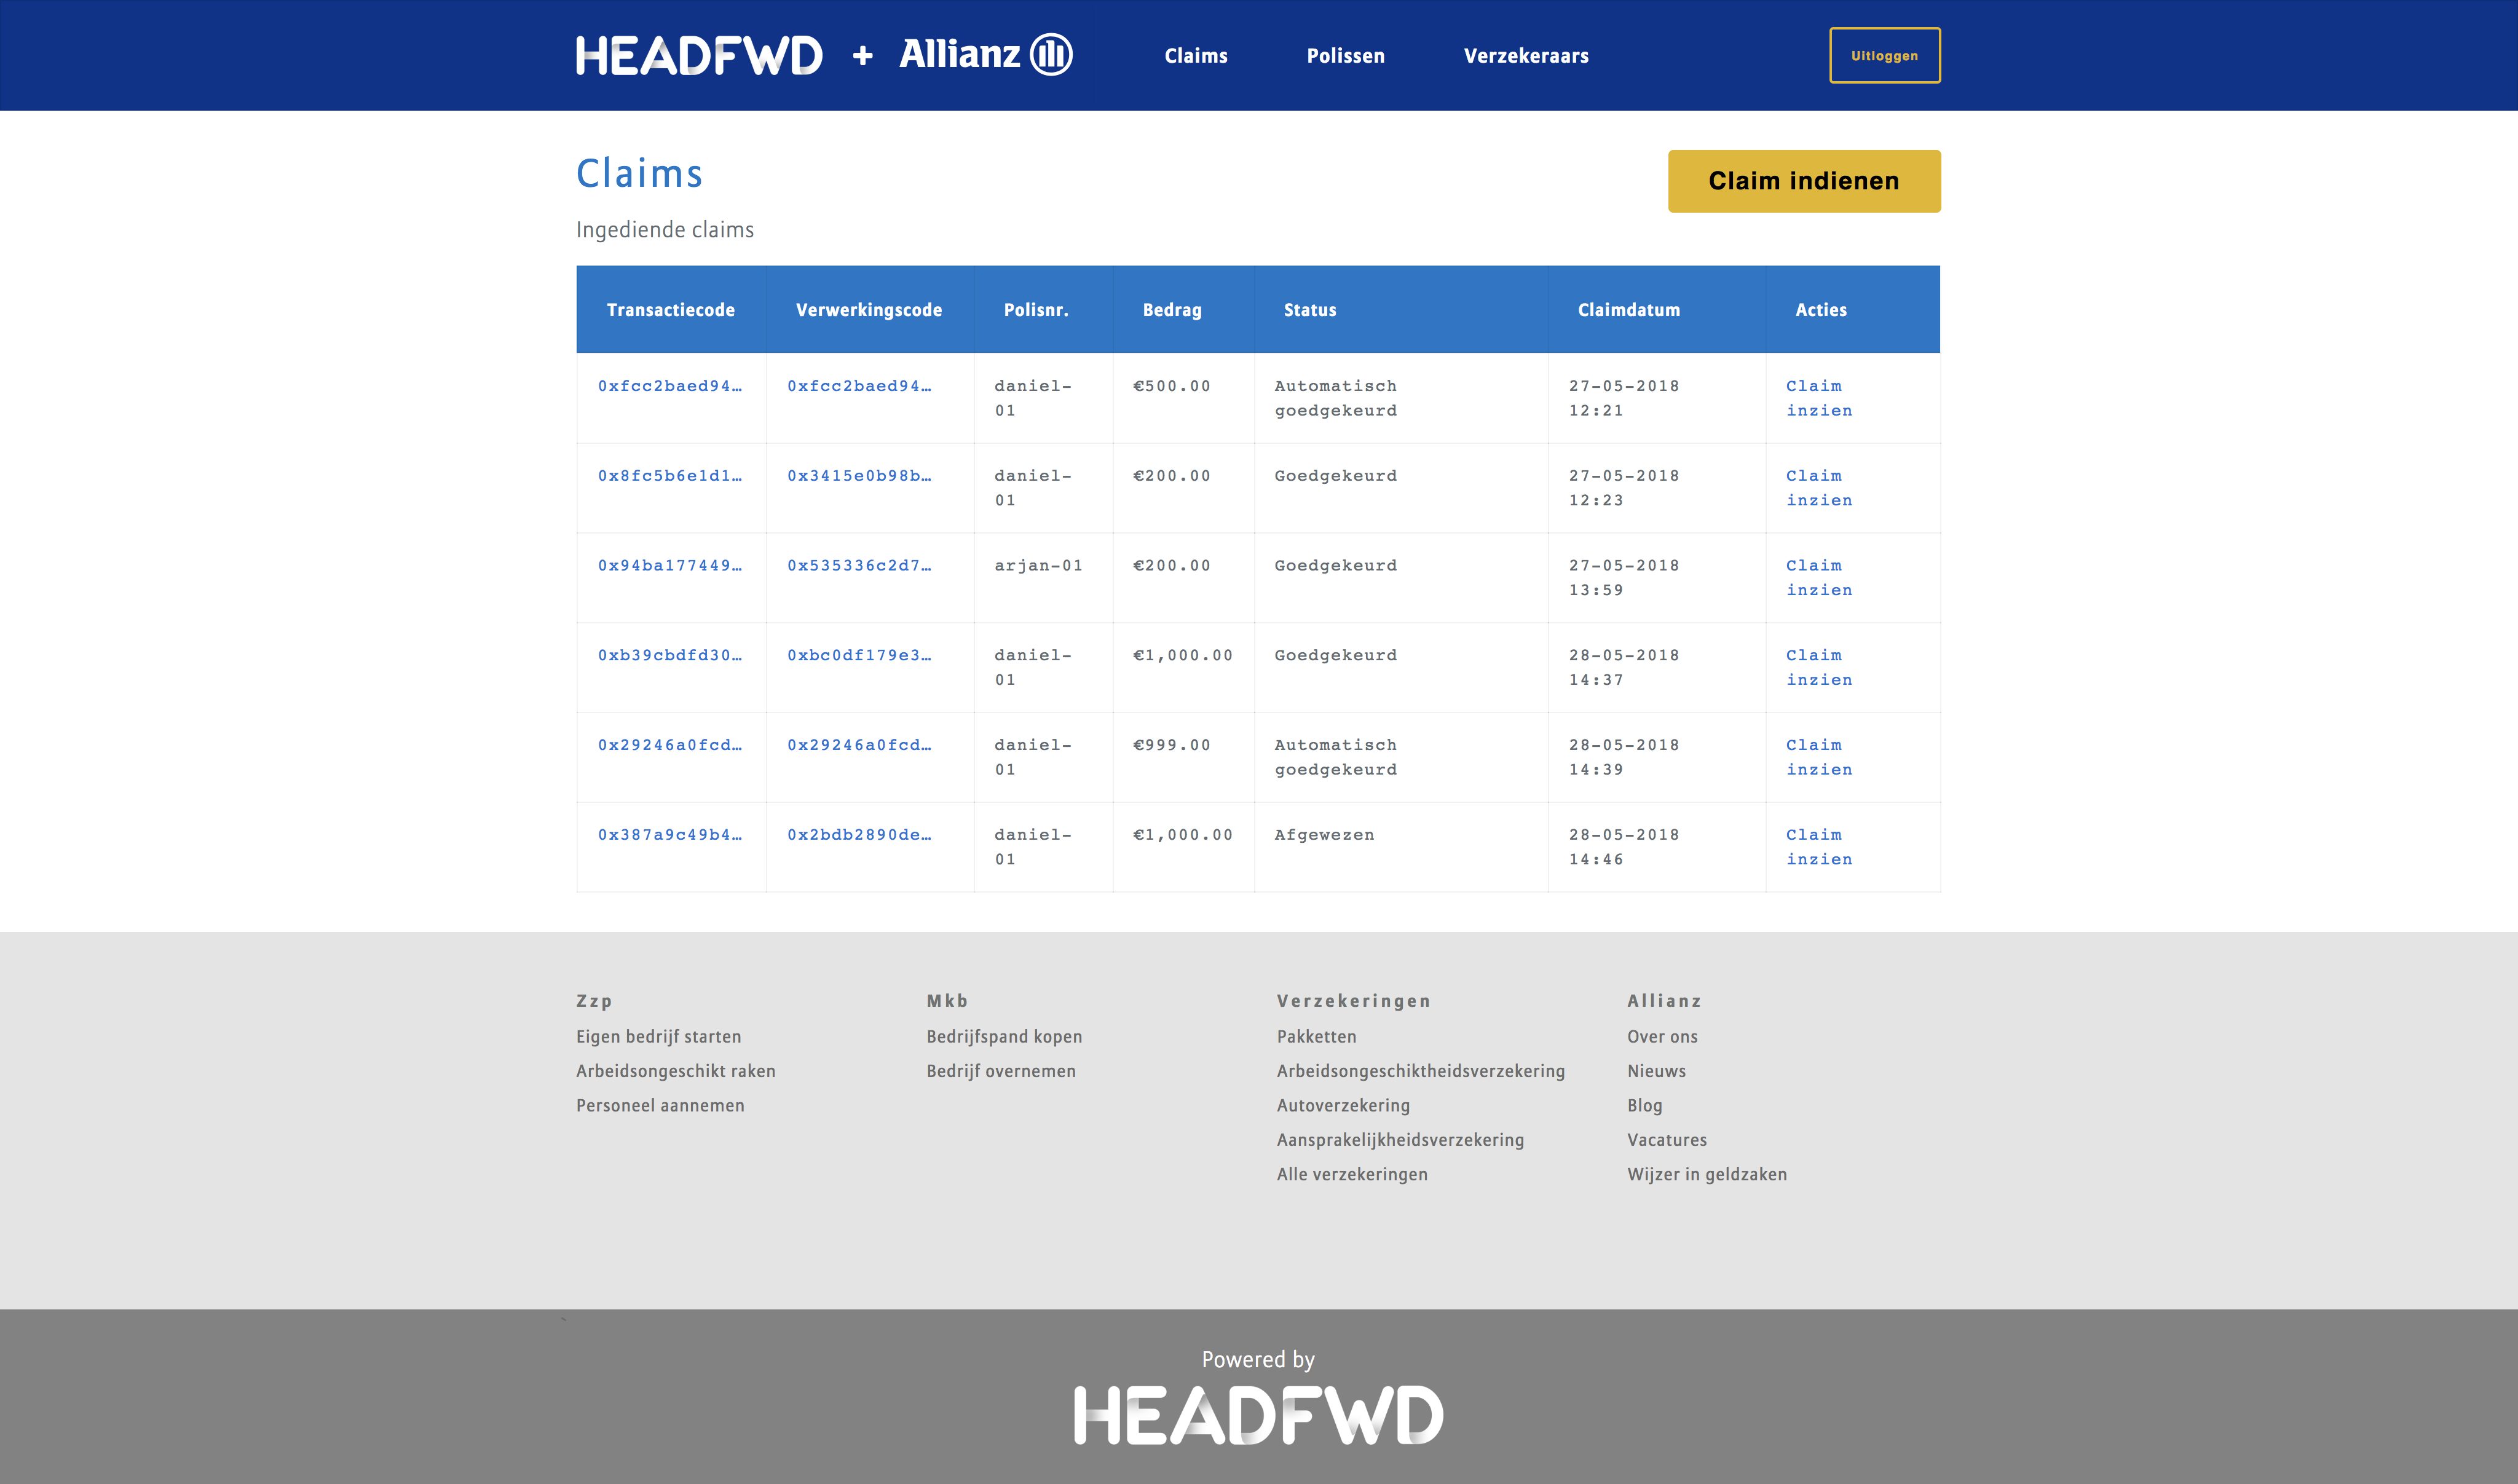
\includegraphics[width=\paperwidth-200]{images/claim-list}
        \caption{Foto van de user interface waar een lijst aan claims te zien is}
        \label{fig:claim-list}
    \end{center}
\end{figure}
Alle musts en zelf een aantals coulds uit de MoScow analyse zijn gerealiseerd. Zo kan bijvoorbeeld ingesteld worden dat om een bepaald claimbedrag een claim automatisch geaccepteerd wordt. Maar deze berekening wordt door iedere lid van het netwerk uitgevoerd.